% Template for Cogsci submission with R Markdown

% Stuff changed from original Markdown PLOS Template
\documentclass[10pt, letterpaper]{article}

\usepackage{cogsci}
\usepackage{pslatex}
\usepackage{float}
\usepackage{caption}

% amsmath package, useful for mathematical formulas
\usepackage{amsmath}

% amssymb package, useful for mathematical symbols
\usepackage{amssymb}

% hyperref package, useful for hyperlinks
\usepackage{hyperref}

% graphicx package, useful for including eps and pdf graphics
% include graphics with the command \includegraphics
\usepackage{graphicx}

% Sweave(-like)
\usepackage{fancyvrb}
\DefineVerbatimEnvironment{Sinput}{Verbatim}{fontshape=sl}
\DefineVerbatimEnvironment{Soutput}{Verbatim}{}
\DefineVerbatimEnvironment{Scode}{Verbatim}{fontshape=sl}
\newenvironment{Schunk}{}{}
\DefineVerbatimEnvironment{Code}{Verbatim}{}
\DefineVerbatimEnvironment{CodeInput}{Verbatim}{fontshape=sl}
\DefineVerbatimEnvironment{CodeOutput}{Verbatim}{}
\newenvironment{CodeChunk}{}{}

% cite package, to clean up citations in the main text. Do not remove.
\usepackage{apacite}

% KM added 1/4/18 to allow control of blind submission


\usepackage{color}

% Use doublespacing - comment out for single spacing
%\usepackage{setspace}
%\doublespacing


% % Text layout
% \topmargin 0.0cm
% \oddsidemargin 0.5cm
% \evensidemargin 0.5cm
% \textwidth 16cm
% \textheight 21cm

\title{Broad consistency but cross-lingusitic variation in the distribution of
information in sentences}


\author{Josef Klafka \and Daniel Yurovsky \\
        \texttt{jklafka@andrew.cmu.edu} and \texttt{yurovsky@cmu.edu} \\
       Department of Psychology \\ Carnegie Mellon University}

\begin{document}

\maketitle

\begin{abstract}
Optimal coding theories of language predict that speakers should keep
the amount of information in their utterances relatively uniform under
the constraints imposed by their language. But how much of a role do
these constraints provide, and does it vary across languages? We find a
consistent non-uniform shape that characterizes both spoken and written
sentences of English that is tempered by predictive context. We then
show that other languages are also characterized by consistent but
non-English shaped curves related to their typological features, but
that sufficient context produces more uniform shapes across languages.
Thus, producers of language appear to structure their utterances in
similar near-uniform ways despite varying linguistic contraints.

\textbf{Keywords:}
information theory; efficient communication; language typology
\end{abstract}

\hypertarget{introduction}{%
\section{Introduction}\label{introduction}}

We use language for a variety of purposes like greeting friends, making
records, and signaling group identity. These purposes all share a common
goal: Transmitting information that changes the mental state of the
listener (Austin, 1975). For this reason, language can be thought of as
a code, one that allows speakers to turn their intended meaning into a
message that can be transmitted to a listener, and subsequently
converted by the listener back into an approximation of the intended
meaning (Shannon, 1948). How should we expect this code to be
structured?

If language has evolved to be a code for information transmission, its
structure should reflect this process of optimization (Anderson \&
Milson, 1989). The optimal code would have to work with two competing
pressures: (1) For listeners to easily and successfully decode messages
sent by the speaker, and (2) For speakers to easily code their messages
and transmit them with minimal effort and error. A fundamental
constraint on both of these processes is the linear order of spoken
language--sounds are produced one at a time and each is unavailable
perceptually once it is no longer being produced.

Humans accomodate this linear order constraint through incremental
processing. People process speech continuously as it arrives, predicting
upcoming words and building expectations about the likely meaning of
utterances in real-time rather than at their conclusion (Kutas \&
Federmeier, 2011; Pickering \& Garrod, 2013; Tanenhaus, Spivey-Knowlton,
Eberhard, \& Sedivy, 1995). Since prediction errors can lead to severe
processing costs and difficulty integrating new information on the part
of listeners, speakers should seek to minimize the chance of prediction
errors when choosing what to say. However, the cost of producing more
predictable utterances and thus minimizing the likelihood of errors is
using more words. Therefore the optimal strategy for speakers seeking to
minimize their production costs is to produce utterances that are just
at the prediction capacity of listeners without exceeding this capacity
(Aylett \& Turk, 2004; Genzel \& Charniak, 2002). In other words,
speakers should consistently transmit information as close to the
listener's fastest decoding rate as possible.

This Uniform Information Density hypothesis has found support at a
variety of levels of language from the structure of individual words to
the syntactic structure of utterances (Jaeger \& Levy, 2007; Piantadosi,
Tily, \& Gibson, 2011; see Gibson et al., 2019 for a review). Further,
speakers make online word choices that smooth out the information in
their utterances (Jaeger \& Levy, 2007; Mahowald, Fedorenko, Piantadosi,
\& Gibson, 2013). While speakers can make bottom-up choices such as
controlling which of several near-synonyms they produce or whether to
produce an optional complementizer like ``that,'' they cannot control
the grammatical properties of their language. Properties like canonical
word order impose top-down constraints on how speakers can structure
what they say (e.g.~English speakers obey a subject-verb-object word
order constraint). While speakers may produce utterances as uniform in
information density as their languages will allow, these top-down
constraints may create significant and unique variation across
languages.

How significant are a language's top-down constraints on speakers? Yu,
Cong, Liang, \& Liu (2016) analyzed how the information in words of
English sentences of a fixed length varies with their order in the
sentence (e.g.~first word, second word, etc). They found a surprising
three-step shape where information first rises, then plateaus, and then
sharply rises again at the ends of sentences. They argued that this
non-linear shape may arise from top-down grammatical constraints on
language. We build on these ideas, asking (1) Whether this shape depends
on listener's predictive models, (2) Whether this shape varies across
linguistic contexts, and (3) Whether this shape is broadly
characteristic of a diverse set of languages or varies predictably from
language to language. We find that languages are characterized by
highly-reliable but cross-linguistically variable information structures
that co-vary with top-down linguistic features. Listeners' predictive
coding flattens these shapes across languages, in accord with
predictions of the Uniform Information Density hypothesis.

\hypertarget{study-1-information-in-written-english}{%
\section{Study 1: Information in Written
English}\label{study-1-information-in-written-english}}

The Uniform Information Density Hypothesis predicts that people should
structure their utterances so that the amount of information in each
unit of language remains nearly constant. An influentual early test of
this idea was performed by Genzel \& Charniak (2002), who analyzed the
amount of information in successive sentences of the same text. They
found that the amount of information increased across sentences when
each was considered in isolation. They reasoned that since all prior
sentences provide the context for reading each new sentences, the amount
of total information (context + paragraph) was overall constant for
human readers.

Yu et al. (2016) applied this same logic to analysis of the information
in individual sentences, computing the entropy of each successive word
in an utterance. Surprisingly, they found found a distinctive three-step
distribution for information in a corpus of written English. The first
word of each sentence tended to contain little information; words in the
middle of sentences each contained roughly the same amount of
information, but the final word of each sentence contained much more
information than any other word. They found the same distribution across
sentence lengths, from sentences with \(15\) words to sentences with
\(45\) words. They took this as evidence against the Uniform Information
Density Hypothesis as, unlike Genzel and Charniak's (2002) results,
information plateaud in the middle of sentences rather than increasing
as it did at the beginnings and ends.

We replicate their analysis here, bringing it more in line with Genzel
and Charniak's (2002) methods. While Yu et al. (2016) considered only
the information in each word, we build two different models. The first,
replicating their analysis, considers the information of each word read
in isolation. The second, following Genzel \& Charniak (2002), is a
trigram model that considers the surprisal of each word having read the
prior two words. We take this trigram model as a better proxy for human
reader's processing of these sentences. Finally, we also develop a
method for averaging the curves for sentences of different lengths
together to provide a single typical information curve signature.

\hypertarget{data}{%
\subsection{Data}\label{data}}

Following Yu et al. (2016), we selected the British National Corpus
(BNC) for analysis (British National Corpus Consortium, 2007). The
British National Corpus is \textasciitilde{}100 million word corpus
consisting of spoken (10\%) and written (90\%) English from the late
20th Century.

\hypertarget{pre-processing}{%
\subsection{Pre-processing}\label{pre-processing}}

We began with the XML version of the corpus, and used the
\texttt{justTheWords.xsl} script provided along with the corpus to
produce a text file with one sentence of the corpus on each line.
Compound words (like ``can't'') were combined, and all words were
converted to lowercase before analysis. This produced a corpus of just
over six million utterance of varying lenghts. From these, we excluded
utterances that were too short to allow for reasonable estimation of
information shape (fewer than 5 words), and utterances that were
unusually long (more than 45 words). This exclusion left us with 89.83\%
of the utterances (Fig \ref{fig:bnc-lengths}.

\begin{CodeChunk}
\begin{figure}[tb]

{\centering 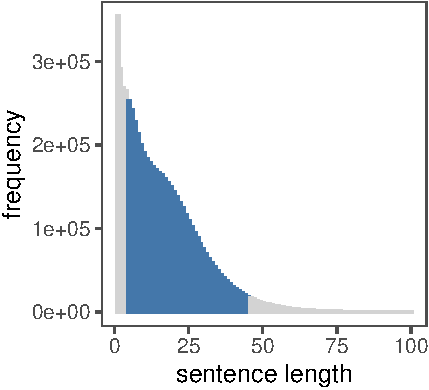
\includegraphics{figs/bnc-lengths-1} 

}

\caption[The distribution of sentence lengths in the British National Corpus]{The distribution of sentence lengths in the British National Corpus. We analyzed sentences of length 5-45 (colored).}\label{fig:bnc-lengths}
\end{figure}
\end{CodeChunk}

\hypertarget{estimating-information}{%
\subsection{Estimating information}\label{estimating-information}}

To estimate how information is distributed across utterances, we
computed the lexical surprisal of each word under two different models
(Levy, 2008; Shannon, 1948). Intuitively, the surprisal of a word is a
measure of how unexpected it would be to read that word, and thus how
much information it contains. First, following Yu et al. (2016), we
estimated a unigram model which considers each word independently,
asking how unexpected that word would be in the absence of any context:
\(\text{surprisal}(\text{word}) = -\log P(\text{word})\). This unigram
surprisal measure is a direct transformation of the word's frequency and
thus less frequent words are more surprising.

Second, we estimated a trigram model in which the surprisal of a given
word (\(w_i\)) encodes how unexpected it is to read it after reading the
prior two words (\(w_{i-1}\) and \(w_{i-2}\)):
\(\text{surprisal}(w_{i}) = -log P(w_i|w_{i-1},w_{i-2})\). This metric
encodes the idea that words that are low frequency in isolation (e.g.
``meatballs'') may become much less surprising in certain contexts (e.g.
``spaghetti and meatballs'') but more surprising in others (e.g.
``coffee with meatballs''). In principle, we would like to encode the
surprisal of a word given all of the prior sentential context
(\(\text{surprisal}(w_{i}) = -P(w_i|w_{i-1}w_{i-2}...w_{1})\). However,
the difficulty of correctly estimating these probabilities from a corpus
grows combinatorically with the number of prior words, and in practice
trigram models perform well as an approximation (see e.g. Chen \&
Goodman, 1999; Smith \& Levy, 2013).

\hypertarget{model-details}{%
\subsubsection{Model details}\label{model-details}}

We estimated the surprisal for each word type in the British National
Corpus using the KenLM toolkit (Heafield, Pouzyrevsky, Clark, \& Koehn,
2013). Each utterance was padded with a special start-of-sentence word
``\(\left<s\right>\)'' and end of sentence word ``\(\left</s\right>\)''.
Trigram estimates did not cross sentence boundaries, so for example the
surprisal of the second word in an utterances was estimated as
(\(\text{surprisal}(w_{2}) = -P(w_2|w_{i},\left<s\right>)\).

Naïve trigram models will underestimate the surprisal of words in
low-frequency trigrams (e.g.~if the word ``meatballs'' appears only once
in the corpus following exactly the words ``spaghetti and'', it is
perfectly predictable from its prior two words). To avoid this
underestimation, we used modified Kneser-Ney smoothing: this method
discounts all ngram frequency counts--reducing the impact of rare ngrams
on probability calculations--and interpolates lower-order ngrams into
the calcuations. These lower-order ngrams are weighted according to the
number of distinct contexts they occur as a continuation (e.g.
``Francisco'' may be a common word in a corpus, but likely only occurs
after ``San'' as in ``San Francisco'', so it receives a lower weighting;
see Chen \& Goodman, 1999).

\hypertarget{averaging-curves}{%
\subsubsection{Averaging curves}\label{averaging-curves}}

To develop a characteristic information curve for sentences in the
corpus, we needed to aggregate sentences that varied dramatically in
length (Fig \ref{bnc-plots}(A)). We used Dynamic Time Warping Barycenter
Averaging (DBA), an algorithm for finding the average of sequences that
share and underlying pattern but vary in length (Petitjean, Ketterlin,
\& Gançarski, 2011). DBA is an extension of standard Dynamic Time
Warping, which searches for an invariant template in shifted and
stretched instances of that template {[}e.g.~all instances of the vowel
`a' in acoustic recordings of a speaker's productions even if the
instances vary in their duration and intensity{]}. DBA inverts this
idea, discovering a latent invariant template from a set of sequences.

We used DBA to discover the short sequence of surprisal values that
characterized the surprisal curves common to sentences of varying
sentence lengths. We first averaged individual sentences of the same
length together, and then applied the DBA algorithm to this set of
average sequences. DBA requires a parameter specifying the length of the
template sequence. We chose 5 as the length of the template sequence
based on our inspection of the curves from the British National Corpus
as well as the curves we found in subsequent studies. However, the
results of this and the following studies were robust to other choices
of this length parameter (7 and 10).

\hypertarget{results-and-discussion}{%
\subsection{Results and Discussion}\label{results-and-discussion}}

\begin{CodeChunk}
\begin{figure}[tb]

{\centering 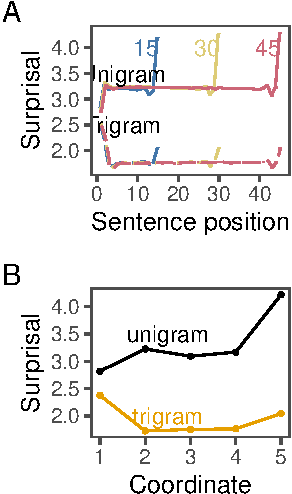
\includegraphics{figs/bnc_plots-1} 

}

\caption[(A) Surprisal by sentence position of length 15, 30, and 45 sentences in the British National Corpus under unigram and trigram surprisal models]{(A) Surprisal by sentence position of length 15, 30, and 45 sentences in the British National Corpus under unigram and trigram surprisal models. Error bars indicate 95\% confidence intervals (tiny due to sample size). (B) Characteristic information curves produced by the DBA algorithm averaging over all sentence lengths in each corpus. }\label{fig:bnc_plots}
\end{figure}
\end{CodeChunk}

We began by replicating Yu et al.'s (2016) analyses, examining the
surprisal of words in sentence of length 15, 30, and 45 estimated by our
unigram model. In line with their computations, we found a reliably
non-linear shape in sentences of all 3 lengths, with the information in
each word rising for the first two words, plateauing in the middle of
sentences, dipping in pen-ultimate position, and rising steeply on the
final word (Fig. \ref{fig:bnc_plots}A).

In comparison, under the trigram model we observed 3 major changes.
First, each word contained significantly less information. This is to be
expected as the knowing two prior words makes it much easier to predict
the next word. Second, the fall and peak at the ends of utterances was
still observable, but much less pronounced. Finally, the first word of
each sentence was now much more surpising than the rest of the words in
the sentence (although still less surprising than the first word under
the unigram model). This is because the model had only the start of
sentence token \(\left<s\right>\) to use as context, but knowing that
the word is the start of an utterance provides some constraints on the
likley word.

Together, these results suggest that Yu et al. (2016) overestimated the
non-uniformity of information in sentences. Because readers of English
beginning a new sentence have read the previous sentence, they can rely
on this context to process the first word (while the model cannot;
Genzel \& Charniak, 2002). Thus, the trigram model likely overestimates
the information for humans reading the first word, which is likely to be
closer in information to words in the middle of the sentence. Second,
the information in the final two words is closer to uniform with the
rest of the sentence than under the trigram model. Nonetheless, the
final words of utterances do consistently contain more information than
the other words.

Finally, Fig. \ref{fig:bnc_plots}B shows the results produced by Dynamic
Time Warping Barycenter Averaging (DBA) on all of the sentences of
varying lengths in the Bristish National Corpus. The algorithm correctly
recovers both the initial and final rise in information under the
unigram model, and the initial fall and smaller final rise in the
trigram model. We take this as evidence that (1) these shapes are
characteristic not just of sentences of length 15, 30, and 45, but of
all lengths, and (2) that DBA effectively recovers the characteristic
structure of utterances of varying lengths.

In sum, the results of Study 1 suggest that sentences of written English
have a characteristic non-uniform information structure, with
information rising at the ends of sentences. This structure is more
pronounced when each word is considered in isolation, but some of the
structure remains even when each word is considered in context. Is this
structure unique to written English, or does it characterize spoken
English as well? In Study 2, we apply this same analysis to two corpora
of spoken English--the first of adults speaking to other adults, and the
second of adults and children speaking to each-other.

\hypertarget{study-2-information-in-spoken-english}{%
\section{Study 2: Information in Spoken
English}\label{study-2-information-in-spoken-english}}

Spoken language is different from written language in several respects.
First, because spoken language isrequires a speaker to produce it, the
speed at which it can be processed is constrained by the speed at which
it is produced. Second, speech occurs in a multimodal environment,
providing listeners information from a variety of sources beyond the
words conveyed (e.g.~prosody, gesture, world context). Finally, the both
words and sentence structures tend to be simpler in spoken language than
written language as they must be produced and processed in real-time
(Christiansen \& Chater, 2016). Thus, sentences of spoken English may
have different information curves than sentences of written English.

The language young children hear is further different from the language
adults speak to each other. Child-directed speech tends to simpler than
adult-directed speech on a number of dimensions including the lengths
and prosodic contours of utterances, the diversity of words, and the
complexity of syntactic structures (Fernald, 1989; Snow, 1972). The
speech produced by young children is even more different from
adult-adult speech, replete with simplifications and modifications
imposed by their developing knowledge of both the lexicon and grammar
(Clark, 2009).

In Study 2, we ask whether spoken English--produced both by adults and
children-- has the same information structure as written English.

\hypertarget{data-1}{%
\subsection{Data}\label{data-1}}

To estimate the information in utterances of adult-adult spoken English,
we used the Santa Barbara Corpus of Spoken American English, \(\sim\)
250,000 word corpus of recordings of naturally occurring spoken
interactions from diverse regions of the United States (Du Bois, Chafe,
Meyer, Thompson, \& Martey, 2000). For parent-child interactions, we
used all of the North American English corpora in the Child Language
Data Exchange System (CHILDES) hosted hosted childes-db (MacWhinney,
2000; Sanchez et al., 2019). We selected for analyses all \(\sim\) 1
million utterances produced by children (mostly under the age of five),
and \(\sim\) 1.7 million utterances produced by the parents of these
children.

\hypertarget{data-processing}{%
\subsection{Data Processing}\label{data-processing}}

All pre-processing and modeling details were identical to Study 1 except
for the selection of sentences for analysis. Because the utterances in
both the Santa Barbara Corpus and CHILDES were significantly shorter
than the sentences in the British National Corpus, we analyzed all
utterances of at least 5 and most 15 words (see Fig.
\ref{fig:spoken_figs}(A)). Models were estimated separately for each of
the 3 corpora.

\hypertarget{results-and-discussion-1}{%
\subsection{Results and Discussion}\label{results-and-discussion-1}}

The information curves found in adults-adult utterances were quite
similar to those of parent-child utterances and child-parent utterances
(Fig. \ref{fig:spoken_figs}B). Under the unigram model, information rose
steeply in the beginnings of utterances, was relatively flatter in the
middle of utterances, and the rose even more steeply at the ends. Under
the trigram model, the first parts words of sentences contained the most
information, information was relatively constant in the middle of
utterances, and then rose slightly again at the ends.

Unfortunately, we we cannot compare the amount of information in each
word across corpora--surprisal is highly correlated with corpus size
(e.g.~there is less information in adults' speech in Santa Babara than
in children's speech in CHILDES). However, we can compare the shapes of
these curves both to each-other and to the written English sentences in
Study 1 \ref{fig:bnc_plots}B. All of these curves appeared to share
their important qualitative features, including the sharp rise at the
end under the unigram model and the attenuation of this rise under the
trigram model. There are small differences--such as the flatter shape in
the middle of written sentences than spoken utterances, but this
difference is pronounced in the utterances of the Santa Barbara corpus
relative to utterances of parents in CHILDES, suggesting that it may be
partly a function of corpus size.

Thus, English--both writen and spoken, both produced by adults and by
children-appears to have a characteristic shape. Are the features of
this shape features of English, or features of language more broadly? In
Study 3 we apply this technique to a diverse set of written languages of
different families to ask whether these structures vary
cross-linguisticly.

\begin{CodeChunk}
\begin{figure*}[tb]

{\centering 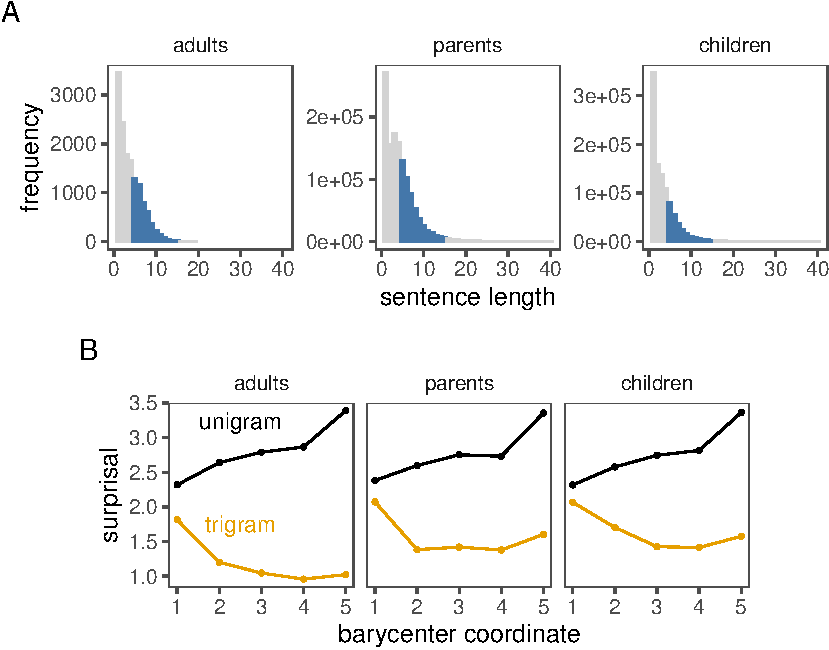
\includegraphics{figs/spoken_figs-1} 

}

\caption[(A) The distribution of sentence lengths in the spoken English corpora]{(A) The distribution of sentence lengths in the spoken English corpora: Adults in Santa Barbara, and parents and children in CHILDES. We analyzed sentences of length 5-15 (colored). (B) Charateristic surprisal curves for these corpora.}\label{fig:spoken_figs}
\end{figure*}
\end{CodeChunk}

\hypertarget{study-3-cross-linguistic-variation-in-information}{%
\section{Study 3: Cross-linguistic variation in
information}\label{study-3-cross-linguistic-variation-in-information}}

\hypertarget{data-2}{%
\subsection{Data}\label{data-2}}

To study cross-linguistic variation in the struture of information
across sentences, we constructed a corpus of Wikipedia articles from all
languages with at least 10,000 articles. This resulted a set of 152
languages from \texttt{n\_fams} families. To examine the relationships
between information curves and linguistic similarity, we used two
meausures of linguistic distance.

To target lexical differences between languages, we used the 40-item
Swadesh word list consisting of basic concepts appearing in all
langauges (Swadesh, 1955; Wichmann et al., 2016). The more similar two
languages' words are, the more similar the two languages are. For each
pair of languages, We computed the average normalized Levenshtein
distance, a string edit distance measure.

To understand the relationship between information curves and
typological features, we used the World Atlas of Language Structures, a
collection of morphological, syntactic, phonological, and other features
of linguistic structure (WALS; Dryer \& Haspelmath, 2013). As WALS is a
compiled database from dozens of papers from different authors, most
features for most languages are fairly sparse. We use a iterative
imputation algorithm for categorical data Multiple Imputation Multiple
Correspondence Analysis to fill in the missing features (MIMCA;
Audigier, Husson, \& Josse, 2017).

\hypertarget{data-processing-1}{%
\subsection{Data processing}\label{data-processing-1}}

All processing was identical to Studies 1 and 2 except for the lengths
of utterances chosen for analyses. To accomodate the variety of lengths
across language corpora, we analyzed sentences of lengths 5 to 30.

\hypertarget{results-and-discussion-2}{%
\subsection{Results and Discussion}\label{results-and-discussion-2}}

Unlike the striking consistency across multiple English corpora, we
found significant variability in the structure of information curves
across languages estimated under the unigram. Fig.
\ref{fig:diff-languages} shows a sample of languages from several
language families. Despite this variability, the shapes of information
curves estimated under the trigram model were more similar
cross-linguistically and to the shapes found in English: Sentences began
with highly informative words (presumably due to lack of context) and
then rapidly approached a uniform level of information. Consistent with
this characterization, pairwise similarities in languages' information
curves estimated under the unigram model were more correlated with their
Swadesh distances (\(r =\) -0.11, \(t =\) -10.27, \(p\) \textless{}
.001) than their distances estimated under the trigram model (\(r =\)
0.03, \(t =\) 2.33, \(p =\) .020).

\begin{CodeChunk}
\begin{figure}[tb]
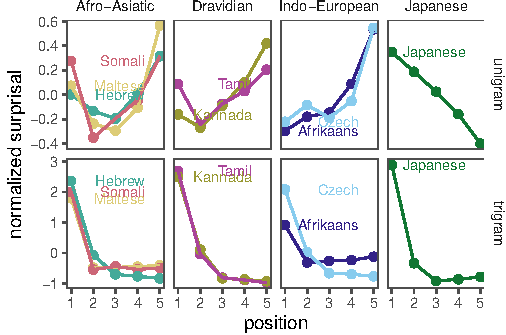
\includegraphics{figs/diff-languages-1} \caption[Characteristic curves for a sample of languages from Wikipedia]{Characteristic curves for a sample of languages from Wikipedia}\label{fig:diff-languages}
\end{figure}
\end{CodeChunk}

While the trigram information curves have a more consistent qualitative
shape, there are differences between languages. The pairwise
similarities between languages' trigram information curves were more
correlated with the number of WALS features they shared (\(r =\) 0.12,
\(t =\) 13.35, \(p\) \textless{} .001) than their similarities estimated
under the trigram model (\(r =\) 0.03, \(t =\) 2.72,\(p =\) .007).

To understand which typological features contribute to these
similarities, we split the WALS features by type: the nominative
categories features describe aspects of morphology such as case systems
and definite/indefinite articles; word order describes the relationship
of the subject, verb, and object to each-other as well as head-modifier
word order; nominative syntax describes noun behavior such as
possessives and adjectives acting as nouns; clauses describes phrasal
and broader sentence syntax; and verb categories describe tense, mood
and aspect as well as morphology on the verb. Fig. \ref{fig:type_cors}
shows the correlation between the similarity of information curves under
both the unigram and trigram models and the number of features of each
of these types two-languages shared. Under the unigram model, word order
features appear to predict information curve similarity. In contrast,
under the trigram model, all features types except for nominative syntax
are reliably correlated with information curve similarity.

\begin{CodeChunk}
\begin{figure}[tb]
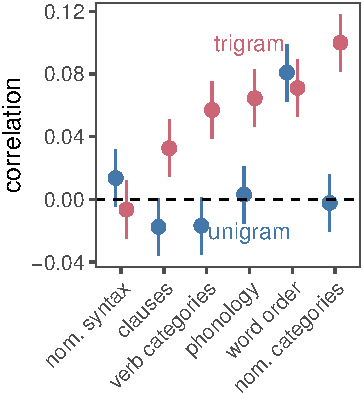
\includegraphics{figs/type_cors-1} \caption[Correlation between info curve and feature similarity]{Correlation between info curve and feature similarity}\label{fig:type_cors}
\end{figure}
\end{CodeChunk}

By considering data from \(159\) diverse languages, we see that the
frequency-based information curves display unique information
distributions for each language. A small part of this cross-linguistic
variation is explicable due to top-down features of the language in
question, such as canonical word order. The majority of the variation
for each language does not derive from top-down features, but we suspect
instead arises from bottom-up choices made by the speakers in each
language.

\hypertarget{conclusion}{%
\section{Conclusion}\label{conclusion}}

In this paper we have proposed a novel method for quantifying
information structure in any language. Our method derives the unique
distribution of information based on word frequency in the language,
irrespective of whether the language in question is spoken or written.
This information structure characterizes the earliest utterances in
child speech all the way to complex sentences in knowledge base entries
by adult writers. The shape of the information distribution in a
language is correlated with the canonical word order in a language, but
is mainly derived from the individual choices speakers make in
communication in a language.

In communication, due to predictive processing, the variation in these
unique frequency-based distributions are washed out. Instead, a uniform
distribution of information emerges across languages, which may allow
listeners to decode information quickly and at a nearly constant rate.
Once they have enough context, listeners optimally decode information.

We average over the surprisal sequences of each length, which obscures
most of the variation in information curve shapes. This may also mean
that there's more bottom-up processing.

\hypertarget{references}{%
\section{References}\label{references}}

\setlength{\parindent}{-0.1in} 
\setlength{\leftskip}{0.125in}

\noindent

\hypertarget{refs}{}
\leavevmode\hypertarget{ref-anderson1989}{}%
Anderson, J. R., \& Milson, R. (1989). Human memory: An adaptive
perspective. \emph{Psychological Review}, \emph{96}(4), 703.

\leavevmode\hypertarget{ref-audigier2017}{}%
Audigier, V., Husson, F., \& Josse, J. (2017). MIMCA: Multiple
imputation for categorical variables with multiple correspondence
analysis. \emph{Statistics and Computing}, \emph{27}(2), 501--518.

\leavevmode\hypertarget{ref-austin1975}{}%
Austin, J. L. (1975). \emph{How to do things with words}. Oxford
university press.

\leavevmode\hypertarget{ref-aylett2004}{}%
Aylett, M., \& Turk, A. (2004). The smooth signal redundancy hypothesis:
A functional explanation for relationships between redundancy, prosodic
prominence, and duration in spontaneous speech. \emph{Language and
Speech}, \emph{47}(1), 31--56.

\leavevmode\hypertarget{ref-british-national-corpus-consortium2007}{}%
British National Corpus Consortium. (2007). \emph{British national
corpus version 3 (BNC XML edition)}. Oxford: Oxford University Computing
Services.

\leavevmode\hypertarget{ref-chen1999}{}%
Chen, S. F., \& Goodman, J. (1999). An empirical study of smoothing
techniques for language modeling. \emph{Computer Speech \& Language},
\emph{13}(4), 359--394.

\leavevmode\hypertarget{ref-christiansen2016}{}%
Christiansen, M. H., \& Chater, N. (2016). The now-or-never bottleneck:
A fundamental constraint on language. \emph{Behavioral and Brain
Sciences}, \emph{39}.

\leavevmode\hypertarget{ref-clark2009}{}%
Clark, E. V. (2009). \emph{First language acquisition}. Cambridge
University Press.

\leavevmode\hypertarget{ref-2013}{}%
Dryer, M. S., \& Haspelmath, M. (Eds.). (2013). \emph{WALS online}.
Leipzig: Max Planck Institute for Evolutionary Anthropology.

\leavevmode\hypertarget{ref-sbc}{}%
Du Bois, J. W., Chafe, W. L., Meyer, C., Thompson, S. A., \& Martey, N.
(2000). Santa barbara corpus of spoken american english. \emph{CD-ROM.
Philadelphia: Linguistic Data Consortium}.

\leavevmode\hypertarget{ref-fernald1989}{}%
Fernald, A. (1989). Intonation and communicative intent in mothers'
speech to infants: Is the melody the message? \emph{Child Development},
1497--1510.

\leavevmode\hypertarget{ref-genzel2002}{}%
Genzel, D., \& Charniak, E. (2002). Entropy rate constancy in text. In
\emph{Proceedings of the 40th annual meeting of the association for
computational linguistics} (pp. 199--206).

\leavevmode\hypertarget{ref-gibson2019}{}%
Gibson, E., Futrell, R., Piandadosi, S. T., Dautriche, I., Mahowald, K.,
Bergen, L., \& Levy, R. (2019). How efficiency shapes human language.
\emph{Trends in Cognitive Sciences}.

\leavevmode\hypertarget{ref-heafield2013}{}%
Heafield, K., Pouzyrevsky, I., Clark, J. H., \& Koehn, P. (2013).
Scalable modified kneser-ney language model estimation. In
\emph{Proceedings of the 51st annual meeting of the association for
computational linguistics (volume 2: Short papers)} (pp. 690--696).

\leavevmode\hypertarget{ref-jaeger2007}{}%
Jaeger, T. F., \& Levy, R. P. (2007). Speakers optimize information
density through syntactic reduction. In \emph{Advances in neural
information processing systems} (pp. 849--856).

\leavevmode\hypertarget{ref-kutas2011}{}%
Kutas, M., \& Federmeier, K. D. (2011). Thirty years and counting:
Finding meaning in the n400 component of the event-related brain
potential (erp). \emph{Annual Review of Psychology}, \emph{62},
621--647.

\leavevmode\hypertarget{ref-levy2008}{}%
Levy, R. (2008). Expectation-based syntactic comprehension.
\emph{Cognition}, \emph{106}(3), 1126--1177.

\leavevmode\hypertarget{ref-macwhinney2000}{}%
MacWhinney, B. (2000). \emph{The childes project: The database} (Vol.
2). Psychology Press.

\leavevmode\hypertarget{ref-mahowald2013}{}%
Mahowald, K., Fedorenko, E., Piantadosi, S. T., \& Gibson, E. (2013).
Info/information theory: Speakers choose shorter words in predictive
contexts. \emph{Cognition}, \emph{126}(2), 313--318.

\leavevmode\hypertarget{ref-petitjean2011}{}%
Petitjean, F., Ketterlin, A., \& Gançarski, P. (2011). A global
averaging method for dynamic time warping, with applications to
clustering. \emph{Pattern Recognition}, \emph{44}(3), 678--693.

\leavevmode\hypertarget{ref-piantadosi2011}{}%
Piantadosi, S. T., Tily, H., \& Gibson, E. (2011). Word lengths are
optimized for efficient communication. \emph{Proceedings of the National
Academy of Sciences}, \emph{108}(9), 3526--3529.

\leavevmode\hypertarget{ref-pickering2013}{}%
Pickering, M. J., \& Garrod, S. (2013). An integrated theory of language
production and comprehension. \emph{Behavioral and Brain Sciences},
\emph{36}(4), 329--347.

\leavevmode\hypertarget{ref-sanchez2019}{}%
Sanchez, A., Meylan, S. C., Braginsky, M., MacDonald, K. E., Yurovsky,
D., \& Frank, M. C. (2019). Childes-db: A flexible and reproducible
interface to the child language data exchange system. \emph{Behavior
Research Methods}, \emph{51}(4), 1928--1941.

\leavevmode\hypertarget{ref-shannon1948}{}%
Shannon, C. E. (1948). A mathematical theory of communication.
\emph{Bell System Technical Journal}, \emph{27}(3), 379--423.

\leavevmode\hypertarget{ref-smith2013}{}%
Smith, N. J., \& Levy, R. (2013). The effect of word predictability on
reading time is logarithmic. \emph{Cognition}, \emph{128}(3), 302--319.

\leavevmode\hypertarget{ref-snow1972}{}%
Snow, C. E. (1972). Mothers' speech to children learning language.
\emph{Child Development}, 549--565.

\leavevmode\hypertarget{ref-swadesh1955}{}%
Swadesh, M. (1955). Towards greater accuracy in lexicostatistic dating.
\emph{International Journal of American Linguistics}, \emph{21}(2),
121--137.

\leavevmode\hypertarget{ref-tanenhaus1995}{}%
Tanenhaus, M. K., Spivey-Knowlton, M. J., Eberhard, K. M., \& Sedivy, J.
C. (1995). Integration of visual and linguistic information in spoken
language comprehension. \emph{Science}, \emph{268}(5217), 1632--1634.

\leavevmode\hypertarget{ref-wichmann2016}{}%
Wichmann, S., Müller, A., Wett, A., Velupillai, V., Bischoffberger, J.,
Brown, C. H., \ldots{} others. (2016). The asjp database. \emph{Max
Planck Institute for the Science of Human History, Jena}.

\leavevmode\hypertarget{ref-yu2016}{}%
Yu, S., Cong, J., Liang, J., \& Liu, H. (2016). The distribution of
information content in english sentences. \emph{arXiv Preprint
arXiv:1609.07681}.

\bibliographystyle{apacite}


\end{document}
